
\section{狄拉克(Dirac)符号}

\begin{frame}
    \frametitle{前情回顾}
    \begin{itemize}
       \done 波动力学
       \done 矩阵力学
       \todo 两者的统一 
    \end{itemize}
        \begin{center}
            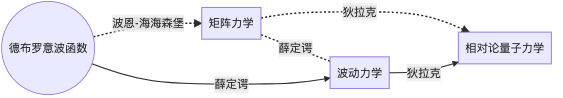
\includegraphics[width=0.9\textwidth]{figs/2021-12-06-16-22-39.png}\\   
        \end{center}    
\end{frame} 

\subsection{左矢与右矢}

\begin{frame}
    量子力学用希尔伯特空间描述,希尔伯特空间是内积空间
    \begin{tcolorbox1}{希尔伯特空间}
    \begin{itemize}
        \item 加法:$\psi + \varphi$
        \item 数乘:$c\psi$
        \item 内积:$(\psi,\psi)$
    \end{itemize}
    \end{tcolorbox1}
    考察内积: $(\psi,\psi)=\int\psi^*\psi d\tau$ \\
    同一波函数放在左边还是右边,意义有所不同: \\
    放右边是线性矢量:  $(\psi,a\psi)=a (\psi,\psi)$ \\
    放左边是反线性矢量:   $(a\psi,\psi)=a^* (\psi,\psi)$   
\end{frame}

\begin{frame}
    \frametitle{左矢和右矢}
    \begin{tcolorbox1}{定义:}
    为了清楚地描述这种线性反线性特点,特定义左矢和右矢
    $$\langle \psi |, \qquad |\psi \rangle $$ 
    内积:\[(\psi,\psi)\equiv \langle \psi | \psi \rangle\]

    有性质: $$\langle a\psi | = \langle \psi |a^* $$
    $$ |a\psi \rangle = a|\psi \rangle$$ 
    \end{tcolorbox1}
\end{frame} 

\begin{frame}
    \frametitle{}
    考察加法和数乘:发现其中的矢量通常是线性的,因此用右矢来代替。\\
    $$\begin{aligned}
    &\text{内积:}   & (\psi,\Psi)  & \qquad\Leftrightarrow \qquad & | \Psi \rangle =\langle \psi | \Psi \rangle \\
    &\text{平均值:}   & \bar{F}=(\Psi,F\Psi)  & \qquad\Leftrightarrow \qquad & \bar{F} =\langle \Psi|F | \Psi \rangle \\
    &\text{态叠加原理:}   & \Psi=a_1 \psi_1+ a_2 \psi_2  & \qquad\Leftrightarrow \qquad &| \Psi \rangle =a_1 |1 \rangle+ a_2 |2 \rangle\\
    &\text{展开式1:}     & \Psi=\sum\limits_{i=1} ^n a_i \psi_i & \qquad \Leftrightarrow \qquad &| \Psi \rangle =\sum\limits_{i=1} ^n a_i |i \rangle\\
    &\text{展开式2:}     & \Psi=\sum\limits_{i=1} ^n (\psi_i ,\Psi) \psi_i & \qquad \Leftrightarrow \qquad &| \Psi \rangle =\sum\limits_{i=1} ^n \langle i | \Psi \rangle |i\rangle\\
    \end{aligned}
    $$
\end{frame} 
 
\subsection{外积}

\begin{frame}
    \frametitle{外积定义}
    考察展开式:
    $$\begin{aligned}
    \Psi \rangle &= \sum\limits_{i=1} ^n \langle i | \Psi \rangle |i\rangle\\
                 &= \sum\limits_{i=1} ^n |i\rangle\langle i | \Psi \rangle \\
    \end{aligned}
    $$
    发现存在:$|i\rangle\langle i$,称为函数的外积,有
    \[\sum\limits_{i=1} ^n |i\rangle\langle i |\]
    称为本征函数系的完全性。
\end{frame} 

\begin{frame}
    \frametitle{外积矩阵表示}
    若:$ \Psi =\sum a_n \varphi_n $\\
    右矢的矩阵形式:
    $$|\Psi\rangle = \begin{pmatrix}
        a_1\\
        a_2\\\
        \cdots\\
        a_n\
    \end{pmatrix}$$ 
    左矢的矩阵形式:
    $$ \langle\Psi| = (a_1 ^*, a_2 ^*, \cdots, a_n ^*) $$
    内积与外积:
    $$\langle\Psi|\Psi\rangle= (a_1 ^*, a_2 ^*, \cdots, a_n ^*) \begin{pmatrix}
        a_1\\
        a_2\\\
        \cdots\\
        a_n\
    \end{pmatrix},\qquad  |\Psi\rangle\langle\Psi|= \begin{pmatrix}
        a_1\\
        a_2\\\
        \cdots\\
        a_n\
    \end{pmatrix} (a_1 ^*, a_2 ^*, \cdots, a_n ^*) $$
\end{frame} 

\begin{frame}
    \frametitle{密度算符}
    定义算符: $ \qquad  \hat{p}_i = |i\rangle\langle i | \qquad $ 有: 
    $$ \hat{p}_i\Psi= |i\rangle\langle i | \Psi \rangle = \langle i | \Psi \rangle |i\rangle=a_i |i\rangle $$
    $$\Psi= \sum\limits_i ^n a_i |i\rangle = \sum\limits_i ^n \hat{p}_i\Psi$$
    可知: $ \hat{p}_i\Psi $ 是矢量$\Psi$ 在第$i$ 个本征矢上的投影, 因此称为{\color{red} 投影算符}\\
    一般地,可定义:$\hat{p} = |\Psi\rangle\langle \Psi |$\\
    考察其在$i$态的平均值:
    $$ \begin{aligned}
    \bar{\hat{p}} &=\langle i |\hat{p} | i \rangle \\
               &=\langle i |\Psi\rangle\langle \Psi | i \rangle \\
               &=(\langle i |\Psi\rangle) (\langle \Psi | i \rangle) \\
               &=a_i ^* a_i =\omega_i \\
    \end{aligned} $$
    是概率密度,因此称 $\hat{p} = |\Psi\rangle\langle \Psi |$ 为 {\color{red} 密度算符},也称为测量算符。
\end{frame} 
 
\begin{frame}
    \frametitle{密度矩阵}
    考察平均值公式:\\
    $$ \begin{aligned}
    \bar{\hat{F}} &=\sum\limits_i |a_i|^2 f_i \\
            &=\sum\limits_i \omega_i \langle i |\hat{F}|i \rangle  \\
            &=\sum\limits_{ij} \omega_i \langle i |\hat{F} |j\rangle \langle j| i\rangle  \\
            &=\sum\limits_{ij} \langle j| i\rangle  \omega_i \langle i |\hat{F} |j\rangle  \\
            &=\sum\limits_{j} \langle j | (\sum\limits_{i}| i \rangle  \omega_i \langle i |) \hat{F} |j\rangle  \\
    \end{aligned} $$
    定义密度矩阵:$ \hat{\rho} = \sum\limits_{i}| i \rangle  \omega_i \langle i | $
\end{frame} 
 
\begin{frame}  
    \frametitle{}  得新的平均值公式:
    \begin{tcolorbox1}{平均值公式-3}
         $$ \begin{aligned}
            \bar{\hat{F}}&=\sum\limits_{j} \langle j | \hat{\rho} \hat{F} |j\rangle \\
                &=tr (\hat{\rho} \hat{F} )
        \end{aligned} $$   
    \end{tcolorbox1} 
\end{frame} 
 
\begin{frame}      
    例:求算符$\hat{F}$在 $|\Psi\rangle =\sum\limits_n a_n |n\rangle $上的平均值 \\
    \alert{解:} 先求算符矩阵:
    $$ F_{nm} = \langle n | F |m \rangle  $$
    再求密度矩阵:
    $$ \hat{\rho} = \sum\limits_{n}| n \rangle  a_n ^* a_n \langle n | $$
    对两矩阵的积求迹得平均值
    $$\bar{\hat{F}}=tr (\hat{\rho} \hat{F} )$$
\end{frame} 
 
\subsection{狄拉克量子力学}

\begin{frame}  
    \frametitle{狄拉克量子力学}  
    量子态: $\hspace{1em}|\Psi \rangle, \qquad$ 位置波函数:$\hspace{1em} \langle x |\Psi \rangle$ \\ \vspace{0.2em}
    展开式: $\hspace{1em}|\Psi \rangle =\sum\limits_{n=1} ^n a_n |n \rangle$ \\
    内积:   $\hspace{2em}\langle \varphi | \Psi \rangle = (\varphi, \Psi)= \int \varphi^*\Psi d\tau $ \\  \vspace{0.2em}
    归一化: $\hspace{1em}\langle \Psi | \Psi \rangle = (\Psi, \Psi)= \int \Psi^*\Psi d\tau = 1 $ \\ \vspace{0.2em}
    正交归一: $\langle n | m \rangle = \delta_{nm} $ \\ \vspace{0.2em}
    $ \hspace{5em} \langle \lambda | \lambda' \rangle = \delta(\lambda-\lambda') $\\ \vspace{0.2em}
    表象: $\hspace{2em}\Psi(x)= \langle x | \Psi \rangle$ \\ \vspace{0.2em}
    展开系数: $ a_n= \langle n | \Psi \rangle$ \\ \vspace{0.2em}
    展开系数: $ a_n ^*= \langle \Psi | n \rangle$ \\ \vspace{0.2em}
    平均值:  $\hspace{1em}\bar{F} = \langle \Psi |F | \Psi \rangle$ \\ \vspace{0.2em}
\end{frame} 
 
\begin{frame} 
    矩阵元:  $\hspace{1em}F_{nm} = \langle n |F | m \rangle$ \\ \vspace{0.2em}
    本征方程:$F|n\rangle =f_n |n\rangle$ \\ \vspace{0.2em}
    幺正变换:$S_{m\alpha} =\langle m| \alpha \rangle $ \\ \vspace{0.2em}
    密度算符:$\rho = |\Psi\rangle\langle \Psi | $ \\ \vspace{0.2em}
    密度矩阵: $\hat{\rho} = \sum\limits_{i}| i \rangle  \omega_i \langle i | $ \\ \vspace{0.2em}
    薛定谔方程:$$ i\hbar \frac{\partial }{\partial t} |\Psi(t)\rangle = H|\Psi(t)\rangle $$ 
    算符运动方程:$$ \frac{d\bar{A}(t)}{dt}=\overline{(\frac{\partial A(t) }{\partial t})}  +\frac{1}{i\hbar} \overline{[A(t),H(t)]}$$
\end{frame} 
 
\begin{frame} 
    \frametitle{应用实例}  
    1、求波函数的矩阵表示:  
    $$|\Psi \rangle =\sum\limits_{n=1} ^n a_n |n \rangle$$
    $$ a_n= \langle n | \Psi \rangle$$ 
    展开系数构成矩阵表示:  
    $$\begin{pmatrix}
    a_1\\
    a_2\\\
    \cdots\\
    a_n\
    \end{pmatrix} $$
\end{frame} 

\begin{frame} 
    \frametitle{}  
    2、求算符的矩阵表示:  
    $$|\varphi \rangle = F |\Psi \rangle$$
    $$|\varphi \rangle = \sum_n F |n\rangle\langle n |\Psi \rangle$$
    $$\langle m |\varphi \rangle = \sum_n  \langle m| F |n\rangle\langle n |\Psi \rangle$$
    $$ b_m = \sum_n  F_{mn} a_n$$

    取遍$n,m$:  
    $$\begin{pmatrix}
    b_1\\
    b_2\\\
    \cdots\\
    b_n\
    \end{pmatrix} 
    = 
    \begin{pmatrix}
        F_{11} & F_{12} & \cdots & F_{1n} \\
        F_{21} & F_{22} & \cdots & F_{2n} \\
        \cdots & \cdots &  \cdots &  \cdots \\
        F_{n1} & F_{n2} & \cdots & F_{nn} \\
    \end{pmatrix} 
    \begin{pmatrix}
        a_1\\
        a_2\\\
        \cdots\\
        a_n\
    \end{pmatrix} 
    $$
\end{frame} 

\begin{frame} 
    3、求薛定谔方程的矩阵表示: 
    $$ \begin{aligned}
    i \hbar \frac{\partial}{\partial t} |\Psi \rangle &= H |\Psi \rangle  \\
    i \hbar \frac{\partial}{\partial t} \langle m |\Psi \rangle &= \langle m |H |\Psi \rangle \\ 
     &= \sum_n \langle m |H |n\rangle\langle n |\Psi \rangle  \\
     i \hbar \frac{\partial}{\partial t} a_m  &= \sum_n H_{mn} a_n 
    \end{aligned}
    $$
\end{frame} 

\begin{frame} 
    4、求平均值公式的矩阵表示: 
    $$ \begin{aligned}
    \bar{F} &= \langle \Psi |F |\Psi \rangle  \\
    &= \langle \Psi |1 \cdot F \cdot 1 |\Psi \rangle  \\
    &= \sum_{mn} \langle \Psi |m\rangle\langle m |F| n\rangle\langle n |\Psi \rangle  \\
    &= \sum_{mn} a_m ^* F_{mn} a_n 
    \end{aligned}
    $$
\end{frame} 

\begin{frame} 
    5、求两算符积的平均值: 
    $$ \begin{aligned}
    \overline{GF} &= \langle \Psi |GF |\Psi \rangle  \\
    &= \langle \Psi |1 \cdot G \cdot 1 \cdot F \cdot 1 |\Psi \rangle  \\
    &= \sum_{mln} \langle \Psi |m\rangle\langle m |G |l\rangle\langle l| F| n\rangle\langle n |\Psi \rangle  \\
    &= \sum_{mln} a_m ^* G_{ml} F_{ln} a_n 
    \end{aligned}
    $$
\end{frame} 

\section{量子力学绘景(Pictures)}

\begin{frame}  
    \frametitle{三种绘景}
    量子力学二个基本方程:  
    \begin{enumerate}
        \item 薛定谔方程:$$ i\hbar \frac{\partial }{\partial t} |\Psi(t)\rangle = H|\Psi(t)\rangle $$
        \item 算符运动方程:$$ \frac{d\bar{A}(t)}{dt}=\overline{(\frac{\partial A(t) }{\partial t})}  +\frac{1}{i\hbar} \overline{[A(t),H(t)]}$$
    \end{enumerate}
    这个世界到底什么在变?\\
    \begin{itemize}
        \done 薛定谔绘景:只有波函数(态)在变,服从薛定谔方程
        \done 海森堡绘景:只有算符(力学量)在变,服从算符运动方程(海森堡方程)
        \done 狄拉克绘景:波函数和算符都在变,一切都只是幺正变换。
    \end{itemize}
\end{frame} 

\begin{frame}  
    \frametitle{}  
    定义时间演化算符:
    $$ U(t,t_0) |\Psi(t_0)\rangle = |\Psi(t)\rangle  $$
    \alert{分析}:
    (1) 因为 $ U(t_0,t_0) |\Psi(t_0)\rangle = |\Psi(t_0)\rangle  $ \\
     有:$$ U(t_0,t_0)=I $$
    (2):求 $ U(t,t_0)$
    $$ \begin{aligned}
        i\hbar \frac{\partial }{\partial t} |\Psi(t)\rangle &= H|\Psi(t)\rangle  \\
        i\hbar \frac{\partial }{\partial t}  U(t,t_0) |\Psi(t)\rangle &= H U(t,t_0) |\Psi(t)\rangle  \\
        i\hbar \frac{\partial }{\partial t}  U(t,t_0)  &= H U(t,t_0)  \\
        U(t,t_0)  &= e^{-\frac{i}{\hbar} H(t-t_0)}  \\
    \end{aligned} $$
\end{frame} 

\begin{frame}  
    (3):$ U(t,t_0)$是幺正算符
    $$ \begin{aligned}
        U(t,t_0)  &= e^{-\frac{i}{\hbar} H(t-t_0)}  \\
        U^\dagger (t,t_0)  &= e^{\frac{i}{\hbar} H(t-t_0)}  \\
        U^\dagger (t,t_0)U(t,t_0) &= U^\dagger (t,t_0)U(t,t_0) \\
         &=e^{\frac{i}{\hbar} H(t-t_0)-\frac{i}{\hbar} H(t-t_0)} \\
         &=e^0
         &=I
    \end{aligned} $$
    因此,有:
    $$ |\Psi(t)\rangle = U(t,t_0) |\Psi(t_0)\rangle   $$
    对比: 
    $$ |\psi_{(B)}\rangle = S^\dagger |\psi_{(A)}\rangle $$
    可知,波函数随时间的演化服从薛定谔方程,但也只是一种幺正算符。
\end{frame} 

\begin{frame}  
    \frametitle{} 
    (4)分析平均值公式:
    $$ \begin{aligned}
        \bar{F} &= \langle \Psi(t) |F(t_0) | \Psi \rangle(t)  \\
        &= \langle \Psi(t_0) |U^\dagger (t,t_0) |F(t_0) | U(t,t_0) |\Psi(t_0)\rangle   \\
        &= \langle \Psi(t_0) |U^\dagger (t,t_0) F(t_0) U(t,t_0) |\Psi(t_0)\rangle   \\
        &= \langle \Psi(t_0) F(t,t_0) |\Psi(t_0)\rangle   \\
    \end{aligned} $$
     式中,令: $$ F(t,t_0) =U^\dagger (t,t_0) F(t_0) U(t,t_0)$$
     对式:
     $$F'=S^\dagger F S $$
     可知,算符随时间的演化与波函数随时间的演化是等价的,也只是一种幺正算符。
\end{frame} 

\begin{frame}
    \frametitle{}  
    \centering
    \LARGE \color{red} 期中考试! \\
\end{frame}